%%%%%%%%%%%%%%%%%%%%%%%%%%%%%%%%
\section{Supplementary}
%%%%%%%%%%%%%%%%%%%%%%%%%%%%%%%%
%
%###############################
\subsection{Children characteristics} \label{sSA:characteristics}
%###############################
%
Table \ref{tab:characteristics} shows the detailed information of the sampled children. The referred table includes the variable used for the matching procedure, i.e. chronological age, while also additional variables thought to be relevant for our hypothesis. No other variables are included as no known additional comorbidities, beside their hearing impairment, are suspected. Additionally, notice the pure tone average (PTA) data was not collected for the NH children.
%
\begin{table}[h!]
	\centering
	\begin{tabular}{|c|ccccccc|} 
		\hline
		& Gender & Chronological & Device length & Hearing & Etiology & \multicolumn{2}{c |}{PTA (dB.)} \\[0.5ex]
		\cline{7-8}
		Child & & age (y;m) & of use (y;m) & age (y;m) & & unaided & aided \\[0.5ex] 
		\hline\hline
		& \multicolumn{7}{l |}{ \textbf{HI/CI children} } \\
		\rowcolor{gray}
		1 & female & 05;07 & 05;00 & 05;00 & Genetic & 120 & 19 \\
		2 & male & 06;04 & 05;09 & 05;09 & CMV & 106 & 23 \\
		\rowcolor{gray}
		3 & male & 06;07 & 05;10 & 05;10 & Genetic & 114 & 35 \\
		4 & female & 06;10 & 06;00 & 06;00 & Unknown & 120 & 20 \\ 
		\rowcolor{gray}
		5 & female & 07;00 & 06;03 & 06;03 & CMV & 115 & 25 \\ 
		6 & male & 07;00 & 05;08 & 05;08 & Genetic & 93 & 32 \\
		\rowcolor{gray}
		7 & female & 07;00 & 06;08 & 06;08 & Genetic & 117 & 17 \\
		8 & female & 07;00 & 05;05 & 05;05 & Unknown & 112 & 42 \\
		\rowcolor{gray}
		9 & male & 07;00 & 05;05 & 05;05 & CMV & 120 & 15 \\ 
		10 & female & 07;01 & 05;11 & 05;11 & Genetic & 120 & 35 \\		
		\rowcolor{gray}
		11 & male & 07;01 & 05;07 & 05;07 & Genetic & 113 & 42 \\
		12 & male & 07;02 & 06;05 & 06;05 & Genetic & 120 & 37 \\
		\rowcolor{gray}
		13 & male & 07;08 & 06;10 & 06;10 & CMV & 114 & 27 \\
		14 & male & 07;09 & 06;02 & 06;02 & CMV & 120 & 35 \\
		\rowcolor{gray}
		15 & male & 08;07 & 07;10 & 07;10 & CMV & 120 & 33 \\
		16 & male & 08;08 & 09;09 & 09;09 & Genetic & 95 & 27 \\
		
		\hline
		
		& \multicolumn{7}{l |}{ \textbf{NH children} } \\	
		\rowcolor{gray}
		17 & female & 06;05 & n.a. & 06;05 & n.a. & n.a. & n.a.\\
		18 & female & 06;06 & n.a. & 06;06 & n.a. & n.a. & n.a.\\
		\rowcolor{gray}
		19 & female & 06;07 & n.a. & 06;07 & n.a. & n.a. & n.a.\\
		20 & female & 06;09 & n.a. & 06;09 & n.a. & n.a. & n.a.\\
		\rowcolor{gray}
		21 & female & 06;09 & n.a. & 06;09 & n.a. & n.a. & n.a. \\
		22 & male & 06;09 & n.a. & 06;09 & n.a. & n.a. & n.a.\\ 
		\rowcolor{gray}
		23 & male & 06;09 & n.a. & 06;09 & n.a. & n.a. & n.a.\\
		24 & male & 06;10 & n.a. & 06;10 & n.a. & n.a. & n.a.\\
		\rowcolor{gray}
		25 & female & 07;01 & n.a. & 07;01 & n.a. & n.a. & n.a.\\
		26 & male & 07;01 & n.a. & 07;01 & n.a. & n.a. & n.a.\\
		\rowcolor{gray}
		27 & male & 07;04 & n.a. & 07;04 & n.a. & n.a. & n.a.\\
		28 & female & 07;08 & n.a. & 07;08 & n.a. & n.a. & n.a.\\
		\rowcolor{gray}
		29 & male & 07;08 & n.a. & 07;08 & n.a. & n.a. & n.a.\\
		30 & female & 07;09 & n.a. & 07;09 & n.a. & n.a. & n.a.\\ 
		\rowcolor{gray}
		31 & female & 08;00 & n.a. & 08;00 & n.a. & n.a. & n.a.\\
		32 & female & 08;01 & n.a. & 08;01 & n.a. & n.a. & n.a.\\	 
		\hline
		\multicolumn{8}{l}{\footnotesize{(y;m) = (years;months)}} \\
		\multicolumn{8}{l}{\footnotesize{n.a. = not applicable / not available}} \\
	\end{tabular}
	\caption[Characteristics of selected children]{Characteristics of selected children.}
	\label{tab:characteristics}
\end{table}
%
%
%###############################
\newpage
\subsection{Experiment details}
%###############################
%
%-------------------------------
\subsubsection{Transcription task} \label{ssSA:transcription}
%-------------------------------
%
The setting for the transcription task comprised the following steps \citep{Boonen_et_al_2020, Boonen_et_al_2021}:
%
\begin{enumerate} %\itemsep1pt
	\item the listener took a seat in front of a computer screen, located at the campus' computer laboratory.
	%
	\item the listener opened Qualtrics \cite{Qualtrics_2005} and select the transcription task.
	%
	\item the listener read two set of instructions presented on the computer screen about:
	\begin{enumerate}
		\item \textit{how to perform the task},
		\item \textit{the aspects not considered for the task}.
	\end{enumerate}
	%
	\item the listener hear the stimuli through high quality headphones, set at a comfortable volume.
	%
	\item the listener wrote the orthographic transcriptions of the utterances, in a free text field in the software environment. 
	%
\end{enumerate}
%
%
%-------------------------------
\subsubsection{Entropy calculation} \label{ssSA:entropy} 
%-------------------------------
%
The outcome from the transcription task was obtained following a two step procedure \citep{Boonen_et_al_2021}. First, we aligned the participant's orthographic transcriptions, at the utterance level, in a column-like grid structure similar to the one presented in Table \ref{tab:align_example}. This step was repeated for every one of the $6400$ transcriptions. Lastly, we computed the entropy measure of the aligned transcriptions as in \citet{Shannon_1948}: 
%
\begin{equation} \label{eq:entropy}
	H = H(\pmb{p}) = \frac{-\sum_{i=1}^{n} p_{i} \cdot \log_{2}(p_{i})}{\log_{2}(N)}
\end{equation}
%
where $H$ is bounded in the unit interval $[0,1]$, $n$ denotes the number of word occurrences within each utterance, $p_{i}$ the probability of such word occurrence, and $N$ the total number of aligned transcriptions per utterance.
%
\begin{comment}
under DoE literature, the design corresponds to $32$ experimental units with $10$ replicates each, making a total of $320$ experimental runs. Moreover, we register $20$ duplicates (transcriptions) for each run, making a total of $6400$ transcriptions.
\end{comment}
%
\begin{table}[h!]
	\centering
	\begin{tabular}{| c | ccccc | } 
		\hline
		Transcription & \multicolumn{5}{c |}{Utterance} \\ [0.5ex]
		\cline{2-6}
		number & 1 & 2 & 3 & 4 & 5 \\ [0.5ex] 
		\hline\hline
		1 & de & jongen & ziet & een & kikker \\ 
		\rowcolor{gray}
		& the & boy & see & a & frog \\ 
		\hline
		2 & de & jongen & ziet & de & [X] \\
		\rowcolor{gray}
		& the & boy & sees & the & [X] \\ 
		\hline
		3 & de & jongen & zag & [B] & kokkin \\
		\rowcolor{gray}
		& the & boy & saw & [B] & cook \\ 
		\hline
		4 & de & jongen & zag & geen & kikkers \\
		\rowcolor{gray}
		& the & boy & saw & no & frogs \\ 
		\hline
		5 & de & hond & zoekt & een & [X] \\
		\rowcolor{gray}
		& the & dog & searches & a & [X] \\ 
		\hline\hline
		Entropy & $0$ & $0.3109$ & $0.6555$ & $0.8277$ & $1$ \\
		\hline
		\multicolumn{4}{l}{\footnotesize{[B] = blank space, [X] = unidentifiable word}}
	\end{tabular}
	\caption[Alignment and entropy calculation]{Alignment and entropy calculation. Extracted from \citet{Boonen_et_al_2021}, and slightly modified with illustrative purposes.}
	\label{tab:align_example}
\end{table}
%

Entropy was used as a quantification of (dis)agreement between listeners' transcriptions, i.e. utterances yielding a high degree of agreement between transcribers were considered highly intelligible, and therefore registered a lower entropy $\left( H \rightarrow 0 \right)$. In contrast, utterances yielding a low degree of agreement were considered as exhibiting low intelligibility, and therefore registered a higher entropy $\left( H \rightarrow 1 \right)$ \citep{Boonen_et_al_2021, Faes_et_al_2021}. 

To exemplify relevant scenarios for the procedure, we generate the entropy for utterances $2$, $4$ and $5$ present in Table \ref{tab:align_example}. To make the example easy to calculate, we assume our data consisted only of five transcriptions in total ($N=5$).

For the second utterance, we observe that four transcriptions identify it with the word \textit{jongen}, while the last with the word \textit{hond}. Therefore, we registered two word occurrences ($n=2$), with probabilities $\pmb{p} = (p_{1}, p_{2}) = (4/5, 1/5)$, and entropy measure equal to:
%
\begin{align*}
	H &= \frac{-\sum_{i=1}^{2} p_{i} \cdot \log_{2}(p_{i})}{\log_{2}(5)} \\
	%
	&= \frac{- \left[ 0.8 \log_{2}(0.8) + 0.2 \log_{2}(0.2) \right] }{\log_{2}(5)} \\
	%
	&\approx 0.3109
\end{align*} 
%
For the fourth utterance, we observe that two transcriptions identify it with the word \textit{een}, one with \textit{de}, one with \textit{geen}, and one with a blank space [B]. Notice the blank space was not expected in such position, therefore, it was considered as a different word occurrence. As a result, the scenario had four word occurrences ($n=4$), with probabilities $\pmb{p} = (p_{1}, p_{2}, p_{3}, p_{4}) = (2/5, 1/5, 1/5, 1/5)$, and entropy measure equal to:
%
\begin{align*}
	H &= \frac{-\sum_{i=1}^{4} p_{i} \cdot \log_{2}(p_{i})}{\log_{2}(5)} \\
	%
	&= \frac{- \left[ 0.4 \log_{2}(0.4) + 3 \cdot 0.2 \log_{2}(0.2) \right] }{\log_{2}(5)} \\
	%
	&\approx 0.8277
\end{align*} 
%
Finally, for the fifth utterance, we observe that all transcriptions identify it with different words. Notice that when a transcriber did not managed to identify (part of) the complete utterance, (s)he was instructed to write [X]  to replace it. However, if more than one transcriber used [X] for an unidentifiable word, each was considered as being different from one another. The latter is done to avoid the artificial reduction of the entropy measure, as [X] values already indicate the lack of intelligibility of the word. Therefore, for the fifth utterance we registered five word occurrences ($n=5$), with probabilities $\pmb{p} = (p_{1}, \dots, p_{5}) = (1/5, \dots, 1/5)$, and entropy measure equal to:
%
\begin{align*}
	H &= \frac{-\sum_{i=1}^{5} p_{i} \cdot \log_{2}(p_{i})}{\log_{2}(5)} \\
	%
	&= \frac{- 5 \cdot 0.2 \log_{2}(0.2) }{\log_{2}(5)} \\
	%
	&= 1
\end{align*} 
%
%
%###############################
\subsection{About speech intelligibility} \label{sSA:SI}
%###############################
%
As described in the introduction, intelligible speech can be defined as the extent to which the elements in an speaker's acoustic signal, e.g. phonemes or words, can be correctly recovered by a listener \citep{Kent_et_al_1989, Whitehill_et_al_2004, vanHeuven_2008, Freeman_et_al_2017}. More specifically, in the context of the transcription task, speech intelligibility can be inferred from the extent a set of transcribers can identify the word contained in an utterance \cite{Boonen_et_al_2021}.

Therefore in this paper, through the implementation of our proposed model, \textit{speech intelligibility} is interpreted as a latent trait of individuals (hypothetical construct), which underlies the probability of observing a set of entropy replicates; that in turns, describes the ability of transcribers to identify the words in an utterance. Henceforth, statements such \textit{`speech intelligibility is influenced by'} can be read as \textit{`the probability of observing a set of entropy replicates for each individual in the sample is influenced by'}. Similar interpretation can be extended to the (latent) \textit{true} entropy measures. 

Despite this practical approach, we emphasize we did our best to ensure the construct validity of our study, by ensuring the transcription task was well understood and appropriately performed by the transcribers.

We then expect speech intelligibility, as measured by our model, to reflect the (general) intelligibility of speech possessed by individuals, but do not deal with general epistemological considerations on the connection between the two.
%
%
%###############################
\subsection{Sampling bias} \label{sSA:sampling_bias}
%###############################
%
As it happens in most observational, and some experimental studies, ours can also be a potential victim of sampling bias. While stratifying on the selection variables can help to balance the samples, and even `correct' the estimates \cite{Cinelli_et_al_2021, Deffner_et_al_2022}, as we do here by controlling for \textit{hearing age}. Given the sample's selection and matching procedures, we cannot ensure the HI/CI nor the NH groups are representative of their respective populations. 

Nevertheless, we argue that by controlling for other relevant confounders, the qualitative results presented in this study holds. However, we cannot discard the presence of unobservable variables that could bias our results, and in that sense, inferences beyond this particular set of children must be taken with care.
%
%
%###############################
\subsection{Model details} \label{sSA:model_details}
%###############################
%
%-------------------------------
\subsubsection{Variability in the beta-proportion distribution} \label{ssSA:model_variability}
%-------------------------------
%
Figure \ref{fig:BetaProp} shows the implications of different `sample sizes' ($M_{i}$) on the dispersion of the beta-proportion distribution \cite{Kruschke_2015}. The panels show different average entropies: the middle panel assumes $\mu=0.5$, the left $\mu=0.2$, and the right $\mu=0.8$ (as shown by the discontinuous lines).

In all three panels we notice two prevalent pattern: (i) the higher the `sample size', the less dispersed is the distribution, and (ii) as expected from non-linear models, the behavior of the dispersion depends on the location of the distribution, i.e. their average value.

Concerning the first patterns, we expect that if the posterior estimates for $M_{i}$ reach lower values, it would imply the entropy replicates $H^{O}_{bik}$ had high dispersion. In contrast, higher $M_{i}$ estimates would imply a lower dispersion in the replicates. In this particular case, a good comparison point is the number of utterances/replicates. If $M_{i}<10$, it would imply that our effective `sample size' (measuring points) is less than the actual number of replicates, and therefore, we would need more replicates to provide an accurate measure of the (latent) \textit{true} entropy. In contrast, $M_{i}>10$ would imply the opposite.
%
\begin{comment}
	The value we choose for the prior $\theta$ can be thought of this way: It is the number of new flips of the coin that we would need to make us teeter between the new data and the prior belief about $\mu$. If we would only need a few new flips to sway our beliefs, then our prior beliefs should be represented by a small $\theta$. If we would need a large number of new flips to sway us away from our prior beliefs about $\mu$, then our prior beliefs are worth a very large $\theta$ \cite{Kruschke_2015}.
\end{comment}

As a final point, it is important to highlight that as the approach uses the `sample size' parameter to model the replicates' heterogeneity, we are effectively estimating a measurement error model \cite{Carroll_2006} on entropy values.
%
\begin{figure} [!h]
	\centering
	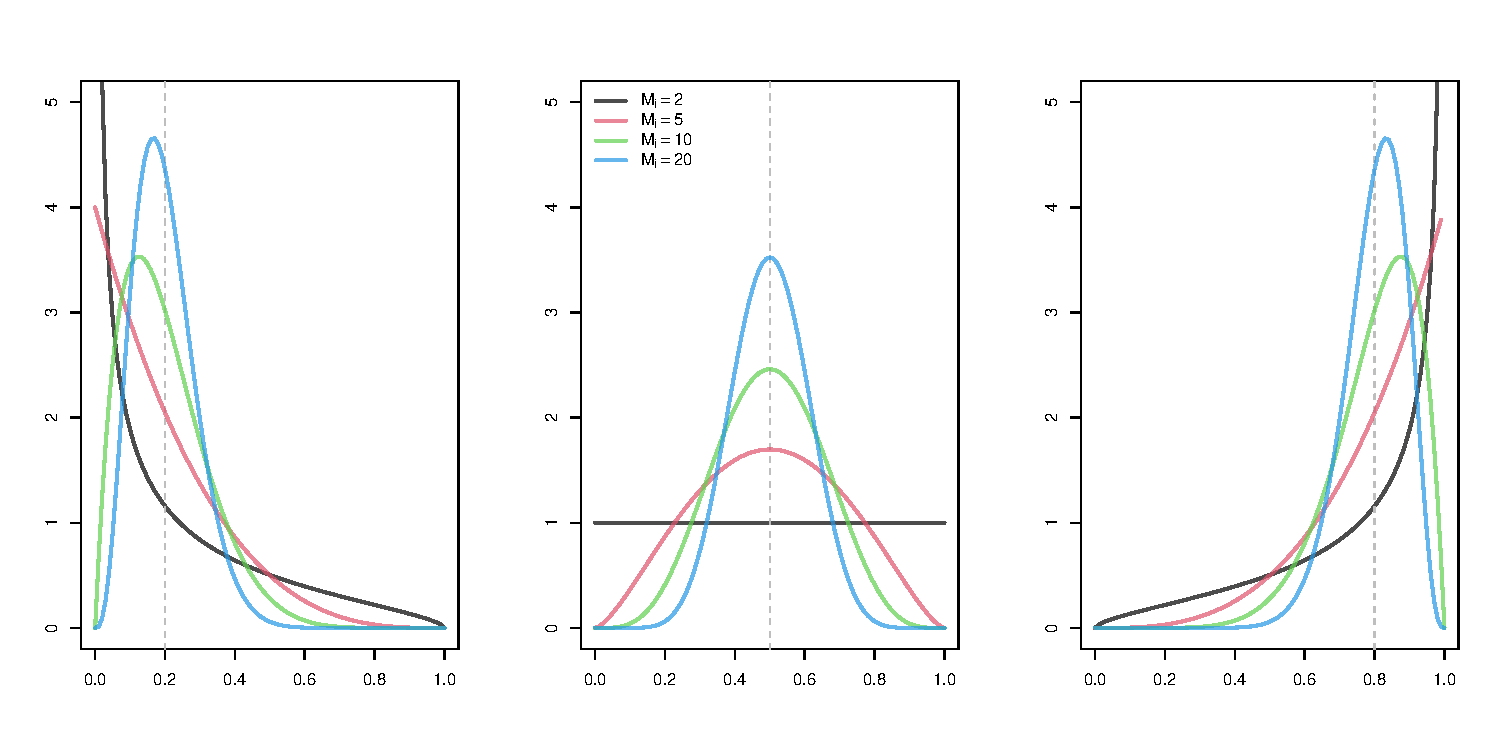
\includegraphics[width=0.9\linewidth]{BetaProp_dist2.pdf}
	\caption[Variability in a beta-proportional distribution]{Variability in a beta-proportional distribution. Discontinuous lines describe the average value for the distribution ($\mu$), solid lines describe the distribution assuming different $\theta = M_{i}$.}
	\label{fig:BetaProp}
\end{figure}
%
%
%-------------------------------
\subsubsection{Data pre-processing} \label{ssSA:preprocessing}
%-------------------------------
%
Besides the exclusion of corrupted observations, e.g. no available transcription, no other information was excluded before the modeling process. This decision departs from what has been done in previous research \cite{Boonen_et_al_2020, vanDaal_2020, Boonen_et_al_2021}. The reason is that we believe the identification of influential observations, through preliminary or univariate procedures, might lead to erroneous exclusion of information, ultimately biasing our results. We believe the identification of \textit{outliers} should not be done outside the context of a full modeling effort \citep{McElreath_2020}, as what can behave as an \textit{outlier} based on a univariate analysis, might behave as expected under the appropriate model.

Considering the previous, instead of eliminating information based on preliminary analysis, we proposed a set of models that can be qualified as \textit{robust} against influential observations. Considering the flexibility of the Bayesian framework, the proposal of such models was a trivial task (see Table \ref{tab:models}).
%
%
%
\begin{figure}[!h]
	\centering
	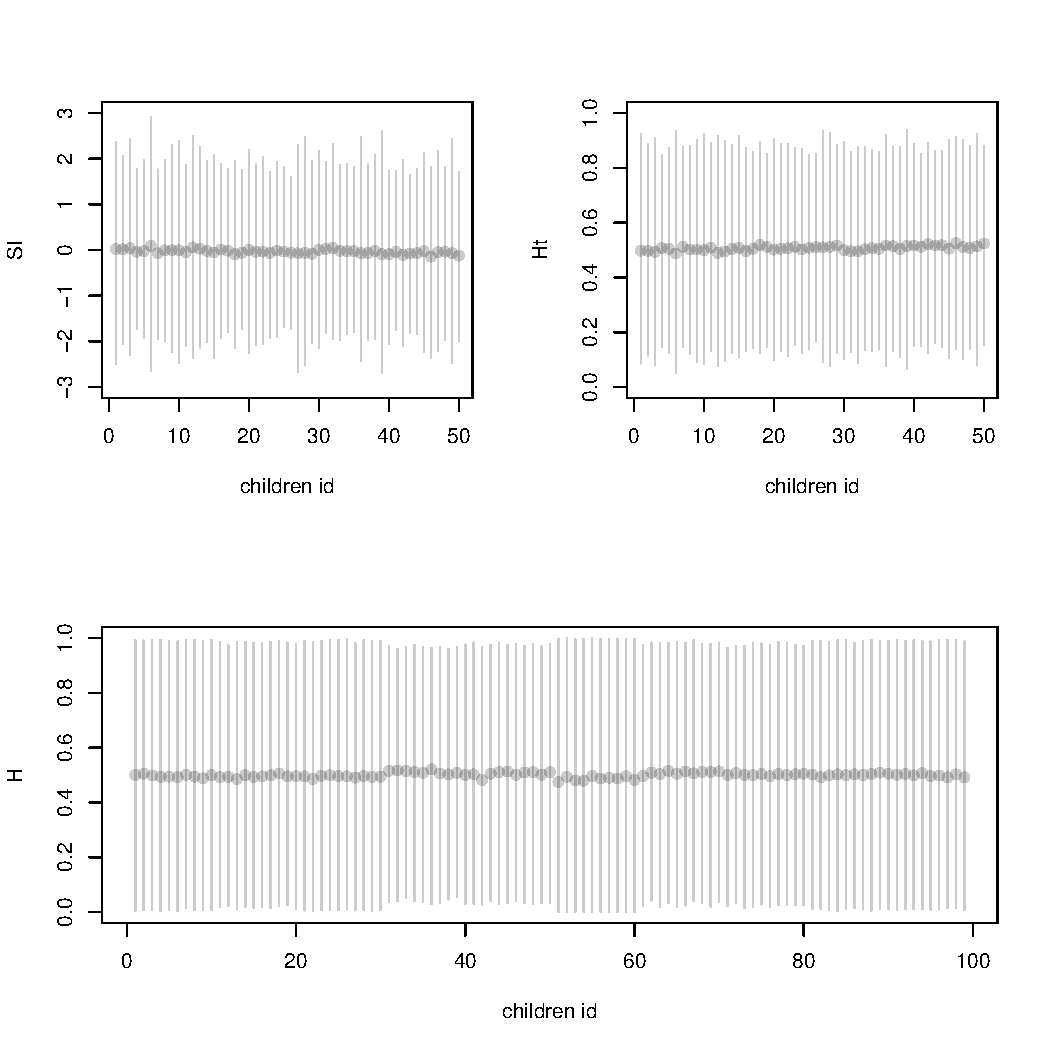
\includegraphics[width=0.6\linewidth]{prior_predictive.pdf}
	\caption[Prior distribution implications]{Prior distribution implications: speech intelligibility, \textit{true} entropy and observed entropy scales. Circles represent mean values, lines depict the $95\%$ compatibility intervals.}
	\label{fig:priors}
\end{figure}
%
%
%-------------------------------
\subsubsection{Priors and hyper-priors}
%-------------------------------
%
For all models, the selection of priors and hyper-priors was done through prior predictive simulation \citep{McElreath_2020}. The selected priors were considered mildly informative and regularizing. 

Figure \ref{fig:priors} shows the implication of our assumptions on the three outcome scales of interest: the \textit{speech intelligibility}, the \textit{true} entropy, and the \textit{observed} entropy replicates. Notice, no undesirable assumption has crept in any of the scales. Consequently, the estimates are free to visit a wide range of results, while also establishing a low probability of reaching impossible outcomes.

Hereby follows a description of the priors for the parameters already defined in section \ref{sS:stat_analysis}:
%
\begin{align}
	%
	M_{i} & \sim \text{Log-Normal}( \mu_{M}, \sigma_{M}) \\
	%
	a_{b} & \sim \text{Normal}(\mu_{b}, \sigma_{b}) \\
	%
	a_{i} & \sim \text{Normal}(\mu_{i}, \sigma_{i}) \\
	%
	\alpha & \sim \text{Normal}(0, 0.2) \\
	%
	\alpha_{E[i],HS[i]} & \sim \text{Normal}(0, 0.3) \\
	%
	\beta_{A, HS[i]} & \sim \text{Normal}(0 , 0.3) \\
	%
	\beta_{P, HS[i]} & \sim \text{Normal}(0, 0.3)
	%
\end{align}

while the hyper-priors were defined as follows:
%
\begin{align}
	%
	\mu_{M} & \sim \text{Normal}(0, 0.5) \\
	%
	\sigma_{M} & \sim \text{Exponential}(1) \\
	%
	\mu_{b} & \sim \text{Normal}(0, 0.2) \\
	%
	\sigma_{b} & \sim \text{Exponential}(1) \\
	%
	\mu_{i} & \sim \text{Normal}(0, 0.2) \\
	%
	\sigma_{i} & \sim \text{Exponential}(1)
	%
\end{align}

\noindent where $\mu_{M}$ represent the average `sample size' and $\sigma_{M}$ the variability of such average. Moreover, $\mu_{b}$ and $\mu_{i}$ represent the average block and children random effect, respectively. Finally, in a similar manner, $\sigma_{b}$ and $\sigma_{i}$ represent the variability present at the blocks and children, respectively (see section \ref{sS:results_variability}).
%
%
%-------------------------------
\subsubsection{Estimation procedure} \label{ssSA:model_estimation}
%-------------------------------
The proposed models in Table \ref{tab:models} were estimated under the Bayesian framework. More specifically, we used the No-U-Turn Hamiltonian Monte Carlo algorithm (No-U-Turn HMC) \citep{Betancourt_et_al_2013, Duane_et_al_1987, Hoffman_et_al_2014, Neal_2012} implemented in \texttt{Stan} \citep{Stan_2020}. We used four chains of $2000$ iterations each, from which the first $1000$ were discarded as a warm-up required by the software, leaving $1000$ effective iterations.

Additionally, all procedures were performed in \texttt{R} 4.1.2 \citep{R_2015} and its integration packages \citep{RStan_2020}, in a 64-bit system with a MINGW 32-bit cross-compiler (\texttt{x86\_64-w64-mingw32/x64}).

\begin{comment}
	\footnote{see \citet{Rivera_2021} (p. 11-13, 15-27) for a detailed description of its benefits and shortcomings.}
\end{comment}
%
%
\begin{figure}[!h]
	\centering
	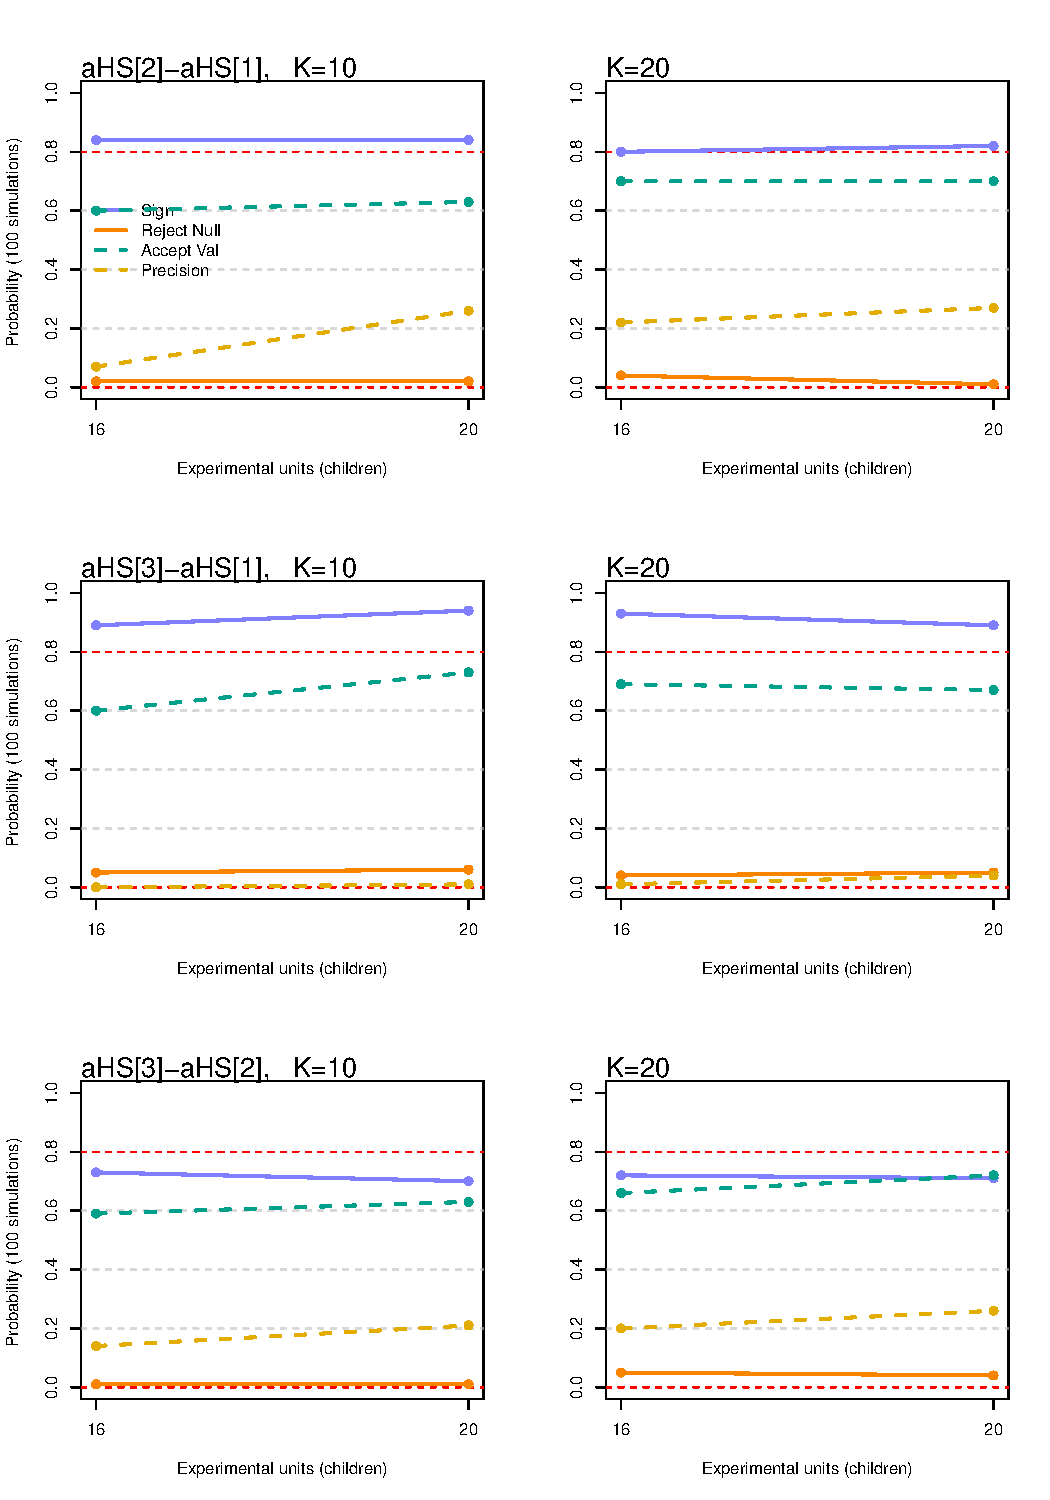
\includegraphics[trim=0 490 0 0, clip, width=0.7\textwidth]{power_result23.pdf}
	%trim=left lower right upper
	\caption[Group contrasts: power on small hearing group differences]{Group contrasts: power on small hearing group differences ($\approx 0.15$)}
	\label{fig:contrasts}
\end{figure}
%
%
%-------------------------------
\subsubsection{Simulation} \label{ssSA:model_simulation}
%-------------------------------
%
Prior to fitting real data, all the proposed models were tested on simulated data. The simulation was done with two purposes: (i) to test the models' ability to recover the `real' parameter values \cite{Fogarty_et_al_2022}, and (ii) to test the power of our data size and assumed hypothesis \cite{Kruschke_2015}. On both instances, we used the \textit{equivalent prior sampling} method \cite{Winkler_1967}, using an idealized data informed by the appropriate children population \cite{DeRaeve_2016}. 

\begin{comment}
	Moreover, we tested three goals\footnote{see \citet{Kruschke_2015} chapter 13 for a detailed overview of the method.}: (a) reject the null value of a parameter, (b) affirm a predicted value, and (c) achieve an estimate precision.
\end{comment}

The results of our simulations highlight two key points. First, regarding the models ability to recover the `real' estimate values, the probabilistic implementations work as intended, i.e. the statistical models manage to recover the `real' values, if enough sample size is available. 

Second, regarding the power of our data to affirm parameter estimates, reject null hypothesis, or provide enough precision for our inferences, three additional points can be made. On the one hand, assuming a small difference among the \textit{hearing status} groups (approximately $0.15$), sixteen children per group are enough to provide at least $60\%$ certainty that our estimates affirm the predicted value, i.e. our model can correctly estimate values different from zero, when such alternative hypothesis is true (see green discontinuous line in figure \ref{fig:contrasts}). Moreover, the previous power threshold surpasses $80\%$ if we assume medium group differences (approximately $0.4$, not shown). Furthermore, in the case of other parameters of interest, even if the assumptions involve small effects (e.g. $bA=0.15$ or $bP=0.1$), our results always show the specific assumed value is tenable with power above $80\%$.

In contrast, the power analysis also reveal that with sufficient amount of variability at the children and replicates levels ($\sigma_{i}=0.5$ and $M_{i}=10$), the models do not have enough power to produce unequivocal null hypothesis rejections (see orange continuous lines in figure \ref{fig:contrasts}), i.e. the compatibility and highest posterior density intervals contain the value of zero, in almost all simulations. The latter implies that with reasonable expectations about the variability between children and the presence of measurement error (multiple replicates to measure one latent value), the statistical models require a data size significantly larger than sixteen children per group. Further model testing indicate that such unequivocal inferences can be accomplished, if we have a sample size similar to the full population size ($70$ children per group).

Lastly, and complementary to the previous result, the statistical precision of our estimates do not achieve power levels above the $80\%$ threshold with our current data size (see yellow discontinuous line in figure \ref{fig:contrasts}). The latter implies that with sixteen children per group, the standard error of our estimates will not allow us to produce definite conclusions, e.g. we will not be certain if the two \textit{hearing status} groups are not different because they are truly not statistically different or because the sample size is not enough to produce unequivocal inferences. This result is also related to the assumptions regarding the variability between children and the presence of measurement error. Similar to the previous case, sufficient levels of precision power can be reached, if we have a sample size similar to the full population size.
%
\begin{comment}
	The results of our simulations indicated that each statistical model was able to recover the `real' parameters values, when the sample size was similar to the population size.
	
	Third and final, no parameter (nor any contrast) managed to reject the null hypothesis or achieve high estimates precision with power above the $80\%$ threshold.
\end{comment}

For more details on the assumed effects and the simulation code, refer to the GitHub repository: \url{https://github.com/jriveraespejo/PhD_UA_paper1}
%
%
%-------------------------------
\subsubsection{Model selection} \label{ssSA:model_selection}
%-------------------------------
%
As stated in previous sections, the current research used the Information-Theoretic Approach \citep{Anderson_2008, Chamberlain_1965} for model selection. The application of the approach required: (i) the expression of the research hypothesis into statistical models, (ii) the selection of the most plausible models, and (iii) to produce inferences based on one or multiple selected models. Since the first step is covered in sections \ref{sS:causal_frame} and \ref{sS:stat_analysis}, and expanded in supplementary section \ref{sSA:model_details}, here we proceed with the intermediate step. 

We used the widely applicable information criterion (WAIC) \citep{Watanabe_2013}, and the Pareto-smoothed importance sampling cross-validation (PSIS) \citep{Vehtari_et_al_2021} as the criteria to select among competing models. Two reasons justify our decision. First, both criteria allow us to use all the information of our Bayesian models, i.e. the posterior distribution of the parameters. Last, and more important, both criteria provide us with the best approximations for the out-of-sample (cross-validated) deviance \citep{McElreath_2020}. The deviance is the best approximation for the Kullback-Liebler (KL) divergence \citep{Kullback_et_al_1951}, i.e. a measure of how far a model is from describing the \textit{true} distribution of our data. In that sense, by comparing the deviance between competing models, we can measure which model is the farthest from `\textit{perfect predictive accuracy}' for our data \cite{McElreath_2020}.

Table \ref{tab:WAIC} and \ref{tab:PSIS} report the criteria for all the proposed models, sorted by the appropriate statistic. Three patterns are visible from the tables. First, we notice that around $63\%$ of the evidence (WE) support two types of models: (a) no interaction and one estimated `sample size', and (b) three (similar) interaction models with one estimated `sample size'. Furthermore, $35\%$ of the evidence is condensed in the diverse types of \textit{robust} models, while the remaining $2\%$ is negligible dispersed in the remaining ones.

Second, comparing the differences in WAIC/PSIS from the `best' model (dWAIC and dPSIS, respectively), we arrive at the same conclusion as the previous paragraph, i.e. the model with no interaction and one estimated `sample size' is the best model, followed by the interaction models with one `sample size', and a bit further away, by the \textit{robust} models. One important point to highlight is that, even when there seem to be a hierarchy of fit among the models, effectively, all of these are indistinguishable from each other, as it can be inferred from their precision estimate (dSE). However, we can also observe, a more precise support for models with any type of interaction and one estimated `sample size', than for the \textit{robust} models.

Third, we observe a greater over-fitting penalty (pWAIC and pPSIS, respectively) for models with a fixed `sample size' than any other model. This is quite particular, as one would expect that a model with less parameters would over-fit less the data. However in this case, it implies the complexity of the data requires more parameters, especially considering there might be some highly influential observations that might sway the estimates of the less parameterized models (see section \ref{sS:results_outliers}). 
%
\begin{table}[h!]
	\centering
	\begin{tabular}{|c|lcccccc|} 
		\hline
		Model & \multicolumn{1}{c}{Name} & WAIC & SE & dWAIC & dSE & pWAIC & WE \\[0.5ex] 
		\hline\hline
		\rowcolor{gray}
		3 & No interaction (one `size') & -621.0 & 42.99 & 0.0 & -- & 31.1 & 0.18 \\
		10 & Full interaction (one `size') & -621.0 & 42.98 & 0.1 & 0.78 & 31.2 & 0.18 \\
		\rowcolor{gray}
		9 & Etiology interaction (one `size') & -620.7 & 43.07 & 0.4 & 0.48 & 31.2 & 0.15 \\
		8 & Age interaction (one `size') & -620.2 & 42.91 & 0.8 & 0.76 & 32.1 & 0.12 \\
		\rowcolor{gray}
		11 & Age interaction (robust) & -620.1 & 42.70 & 0.9 & 2.21 & 34.2 & 0.12 \\
		12 & Etiology interaction (robust) & -619.9 & 42.77 & 1.1 & 2.06 & 34.4 & 0.10 \\
		\rowcolor{gray}
		4 & No interaction (robust) & -619.2 & 42.81 & 1.8 & 2.18 & 34.8 & 0.07 \\
		13 & Full interaction (robust) & -618.8 & 42.65 & 2.2 & 2.17 & 35.0 & 0.06 \\
		\rowcolor{gray}
		5 & Age interaction (fixed `size') & -578.2 & 52.51 & 42.8 & 16.85 & 50.7 & 0.00 \\
		6 & Etiology interaction (fixed `size') & -578.2 & 52.63 & 42.8 & 16.95 & 50.7 & 0.00 \\
		\rowcolor{gray}
		2 & No interaction (fixed `size') & -577.6 & 52.59 & 43.5 & 16.97 & 51.0 & 0.00 \\
		1 & Intercept only (fixed `size') & -576.8 & 52.98 & 44.3 & 17.40 & 51.8 & 0.00 \\
		\rowcolor{gray}
		7 & Full interaction (fixed `size') & -575.8 & 52.58 & 45.3 & 16.96 & 52.1 & 0.00 \\
		\hline\hline
		\multicolumn{1}{|r|}{\small SE} & \multicolumn{7}{l|}{\small WAIC approximate standard error} \\
		\multicolumn{1}{|r|}{\small dWAIC} & \multicolumn{7}{l|}{\small difference in WAIC from the best model} \\
		\multicolumn{1}{|r|}{\small dSE} & \multicolumn{7}{l|}{\small standard error for the difference in WAIC from the best model} \\
		\multicolumn{1}{|r|}{\small pWAIC} & \multicolumn{7}{l|}{\small WAIC over fitting penalty} \\
		\multicolumn{1}{|r|}{\small WE} & \multicolumn{7}{l|}{\small weight of evidence} \\
		\hline
	\end{tabular}
	\caption[Fit of statistical models: WAIC]{Fit of statistical models: WAIC.}
	\label{tab:WAIC}
\end{table}
%
\begin{table}[h!]
	\centering
	\begin{tabular}{|c|lcccccc|} 
		\hline
		Model & \multicolumn{1}{c}{Name} & PSIS & SE & dPSIS & dSE & pPSIS & WE \\[0.5ex] 
		\hline\hline
		\rowcolor{gray}
		3 & No interaction (one `size') & -619.8 & 42.98 & 0.0 & -- & 31.8 & 0.22 \\
		10 & Full interaction (one `size') & -619.7 & 42.97 & 0.0 & 0.82 & 31.8 & 0.22 \\
		\rowcolor{gray}
		9 & Etiology interaction (one `size') & -619.2 & 43.05 & 0.5 & 0.51 & 32.0 & 0.17 \\
		8 & Age interaction (one `size') & -619.0 & 42.89 & 0.7 & 0.81 & 31.8 & 0.15 \\
		\rowcolor{gray}
		11 & Age interaction (robust) & -617.8 & 42.70 & 2.0 & 2.19 & 35.4 & 0.08 \\
		12 & Etiology interaction (robust) & -617.7 & 42.77 & 2.1 & 2.07 & 35.5 & 0.08 \\
		\rowcolor{gray}
		4 & No interaction (robust) & -616.5 & 42.81 & 3.3 & 2.19 & 36.1 & 0.04 \\
		13 & Full interaction (robust) & -616.3 & 42.64 & 3.4 & 2.13 & 36.2 & 0.04 \\
		\rowcolor{gray}
		6 & Etiology interaction (fixed `size') & -576.0 & 52.63 & 43.7 & 17.00 & 51.7 & 0.00 \\
		5 & Age interaction (fixed `size') & -575.9 & 52.54 & 43.9 & 16.94 & 51.9 & 0.00 \\
		\rowcolor{gray}
		2 & No interaction (fixed `size') & -575.3 & 52.59 & 44.4 & 17.03 & 52.1 & 0.00 \\
		1 & Intercept only (fixed `size') & -574.6 & 52.97 & 45.1 & 17.44 & 52.9 & 0.00 \\
		\rowcolor{gray}
		7 & Full interaction (fixed `size') & -573.8 & 52.61 & 46.0 & 17.01 & 53.1 & 0.00 \\
		\hline\hline
		\multicolumn{1}{|r|}{\small SE} & \multicolumn{7}{l|}{\small WAIC approximate standard error} \\
		\multicolumn{1}{|r|}{\small dPSIS} & \multicolumn{7}{l|}{\small difference in PSIS from the best model} \\
		\multicolumn{1}{|r|}{\small dSE} & \multicolumn{7}{l|}{\small standard error for the difference in PSIS from the best model} \\
		\multicolumn{1}{|r|}{\small pPSIS} & \multicolumn{7}{l|}{\small PSIS over fitting penalty} \\
		\multicolumn{1}{|r|}{\small WE} & \multicolumn{7}{l|}{\small weight of evidence} \\
		\hline
	\end{tabular}
	\caption[Fit of statistical models: PSIS]{Fit of statistical models: PSIS.}
	\label{tab:PSIS}
\end{table}
%
%